\subsection{Features}
A wide variety of features can be used to build a classifier for tweets. The most widely used and basic feature set is word n-grams. However, there's a lot of domain specific information present in tweets that can also be used for classifying them. We have experimented with two sets of features:

\subsubsection{Unigrams}
Unigrams are the simplest features that can be used for text classification. A Tweet can be represented by a multiset of words present in it. We, however, have used the presence of unigrams in a tweet as a feature set. Presence of a word is more important than how many times it is repeated. Pang et al. found that presence of unigrams yields better results than repetition \cite{survey}. This also helps us to avoid having to scale the data, which can considerably decrease training time \cite{GBH}. \figref{fig:1grams} illustrated the cumulative distribution of words in our dataset.
%TODO Pang's paper

\begin{figure}[h!]
\centering
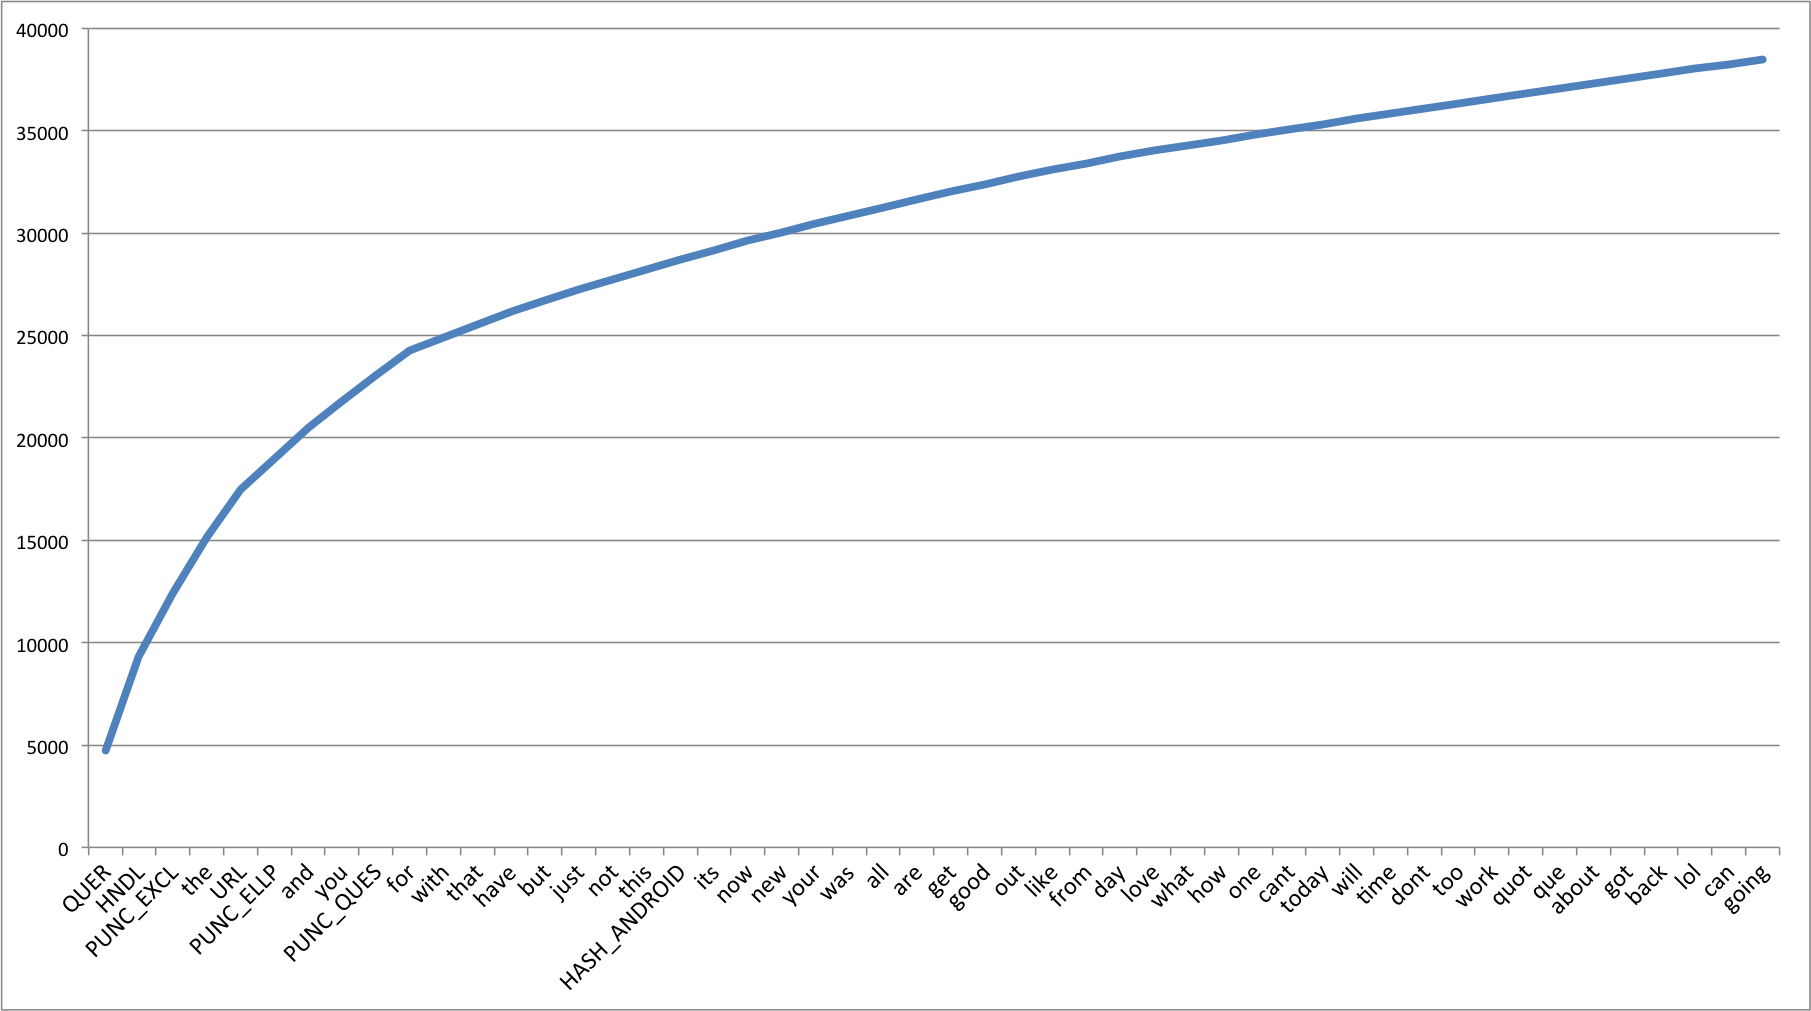
\includegraphics[width=\textwidth]{img/1grams.png}
\caption{Cumulative Frequency Plot for 50 Most Frequent Unigrams}
\label{fig:1grams}
\end{figure}

We also observe that the unigrams nicely follow Zipf’s law. It states that in a corpus of natural language, the frequency of any word is inversely proportional to its rank in the frequency table. \figref{fig:zipf} is a plot of log frequency versus log rank of our dataset. A linear trendline fits well with the data.

\begin{equation}
log( f ) = -0.9799 log( r ) + 3.9838
\end{equation}
\begin{equation}
f = 10^{3.9838} r^{-0.9799}
\end{equation}
\begin{equation}
f \propto \frac{1}{r}
\end{equation}

\begin{figure}[h!]
\centering
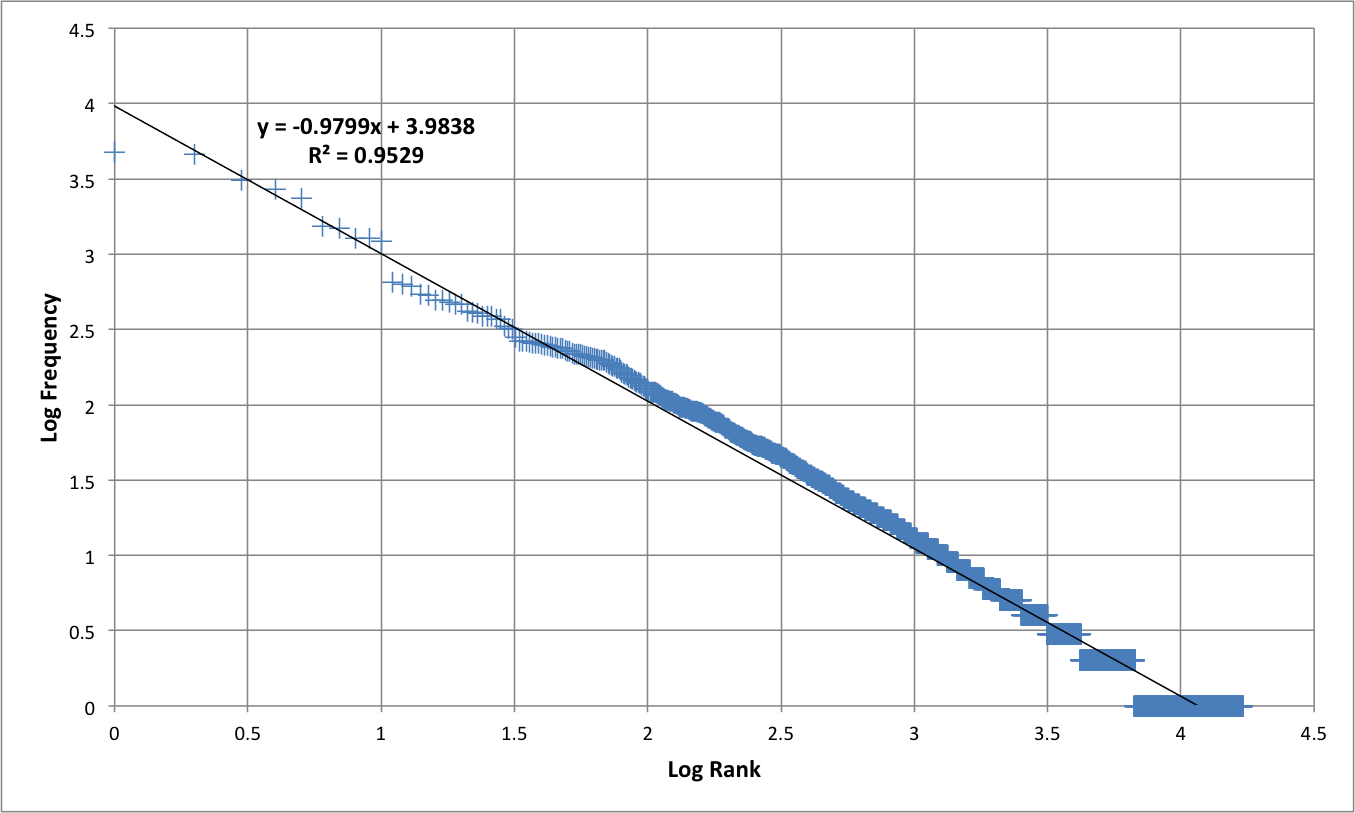
\includegraphics[width=\textwidth]{img/zipfs_law.png}
\caption{Zipf's Law - Log Frequency versus Log Rank plot for unigrams}
\label{fig:zipf}
\end{figure}


\subsubsection{N-grams}
N-gram refers to an n-long sequence of words. Probabilistic Language Models based on Unigrams, Bigrams and Trigrams can be successfully used to predict the next word given a current context of words. In the domain of sentiment analysis, the performance of N-grams is unclear. According to Pang et al., some researchers report that unigrams alone are better than bigrams for classification movie reviews, while some others report that bigrams and trigrams yield better product-review polarity classification \cite{survey}.

As the order of the n-grams increases, they tend to be more and more sparse. Based on our experiments, we find that number of bigrams and trigrams increase much more rapidly than the number of unigrams with the number of Tweets. \figref{fig:ngrams_dist_1} shows the number of n-grams versus number of Tweets. We can observe that bigrams and trigrams increase almost linearly where as unigrams are increasing logarithmically.

\begin{figure}[h!]
\centering
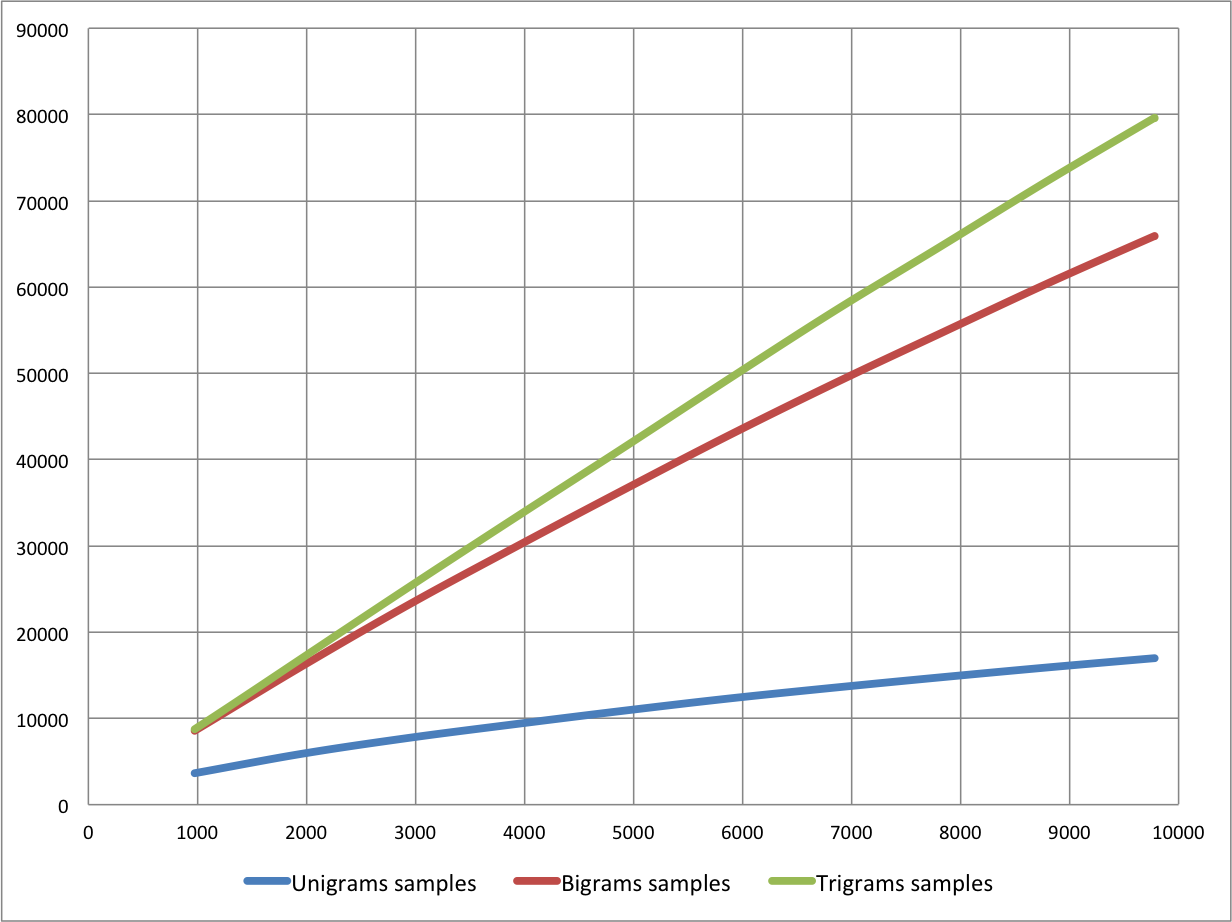
\includegraphics[width=\textwidth]{img/Ngrams_dist_1.png}
\caption{Number of n-grams vs. Number of Tweets}
\label{fig:ngrams_dist_1}
\end{figure}
%TODO: label 'ngrams growth'

Because higher order n-grams are sparsely populated, we decide to trim off the n-grams that are not seen more than once in the training corpus, because chances are that these n-grams are not good indicators of sentiments. After the filtering out non-repeating n-grams, we see that the number of n-grams is considerably decreased and equals the order of unigrams, as shown in \figref{fig:ngrams_dist_2}.

\begin{figure}[h!]
\centering
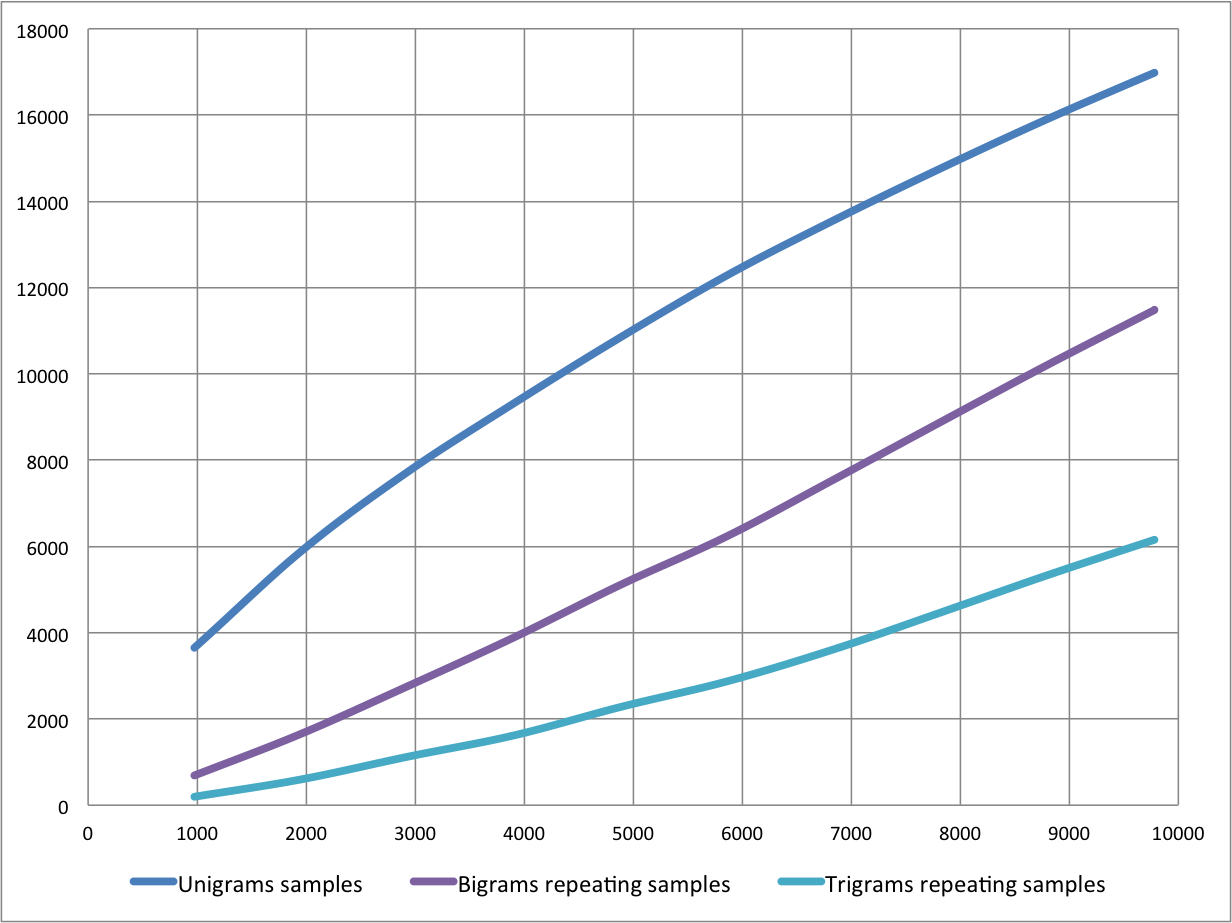
\includegraphics[width=\textwidth]{img/Ngrams_dist_2.png}
\caption{Number of repeating n-grams vs. Number of Tweets}
\label{fig:ngrams_dist_2}
\end{figure}
%TODO: label 'ngrams filtered growth'

\figref{fig:2grams} and \figref{fig:3grams} show the cumulative distribution of the most frequent bigrams and trigrams respectively.

\begin{figure}[h!]
\centering
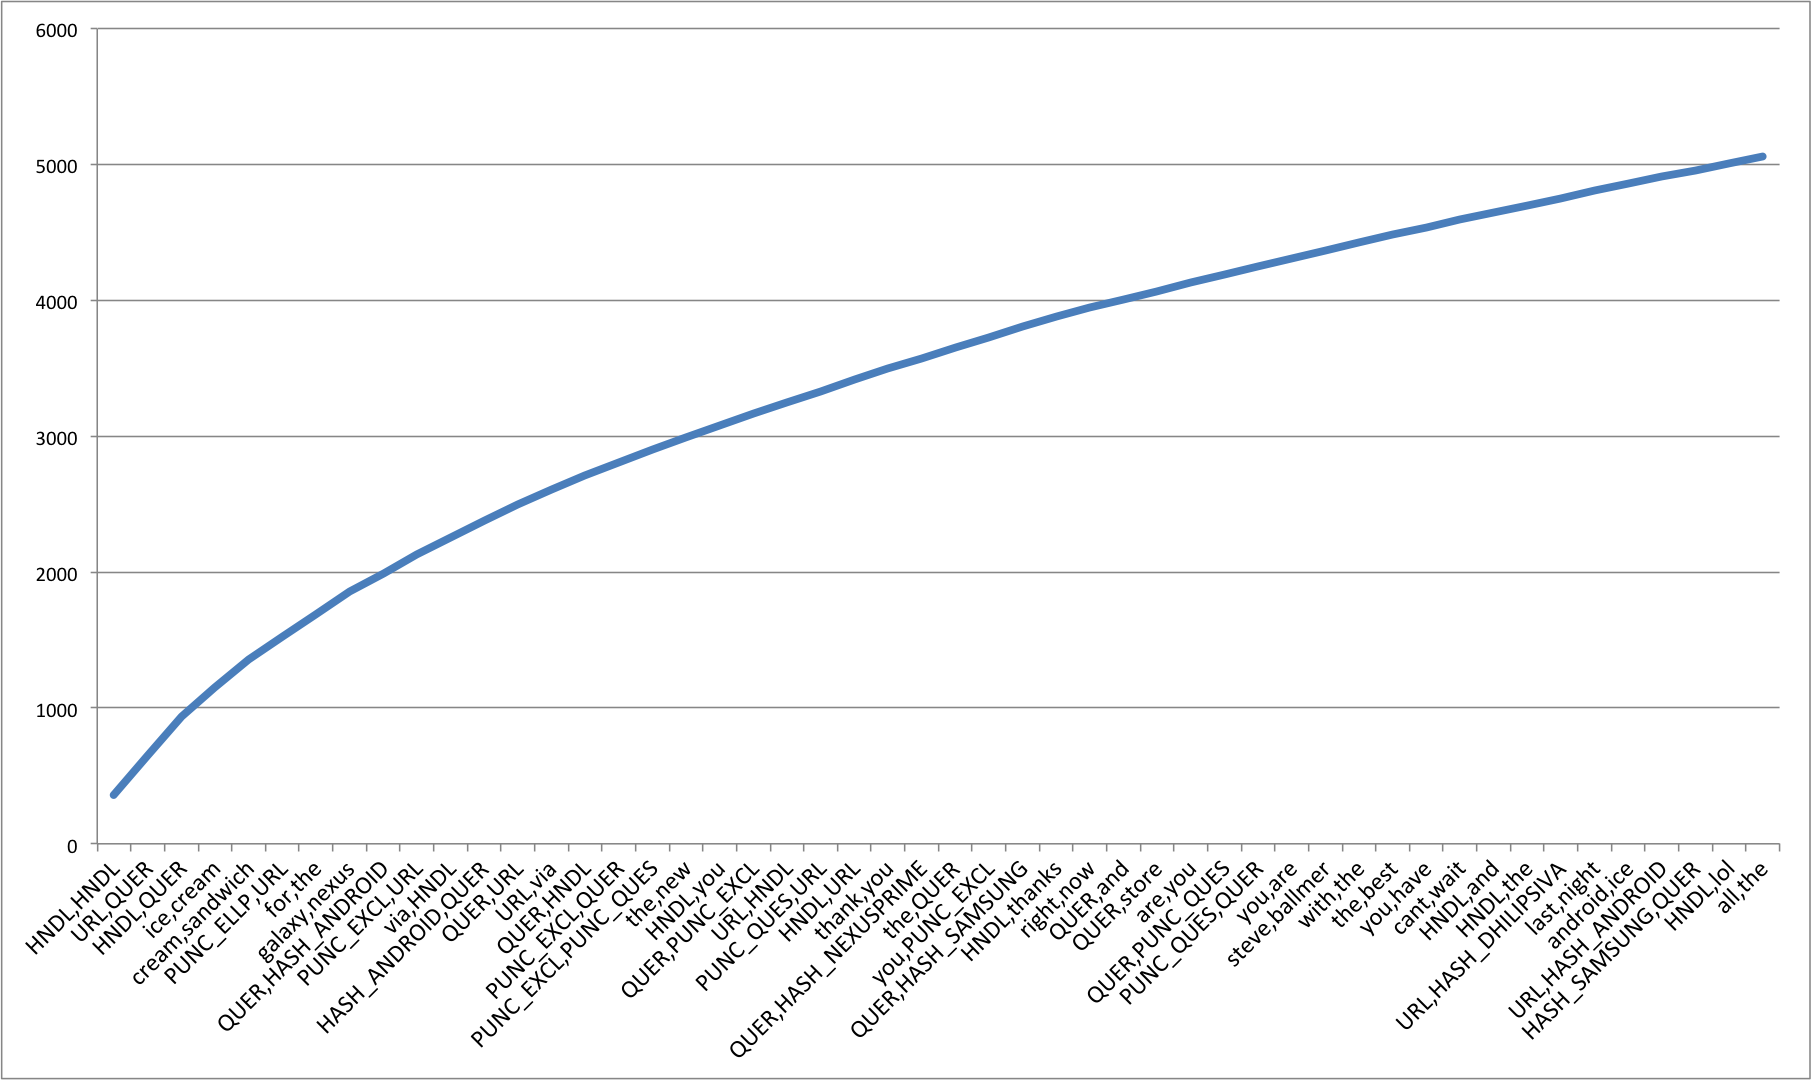
\includegraphics[width=\textwidth]{img/2grams.png}
\caption{Cumulative Frequency Plot for 50 Most Frequent Bigrams}
\label{fig:2grams}
\end{figure}

\begin{figure}[h!]
\centering
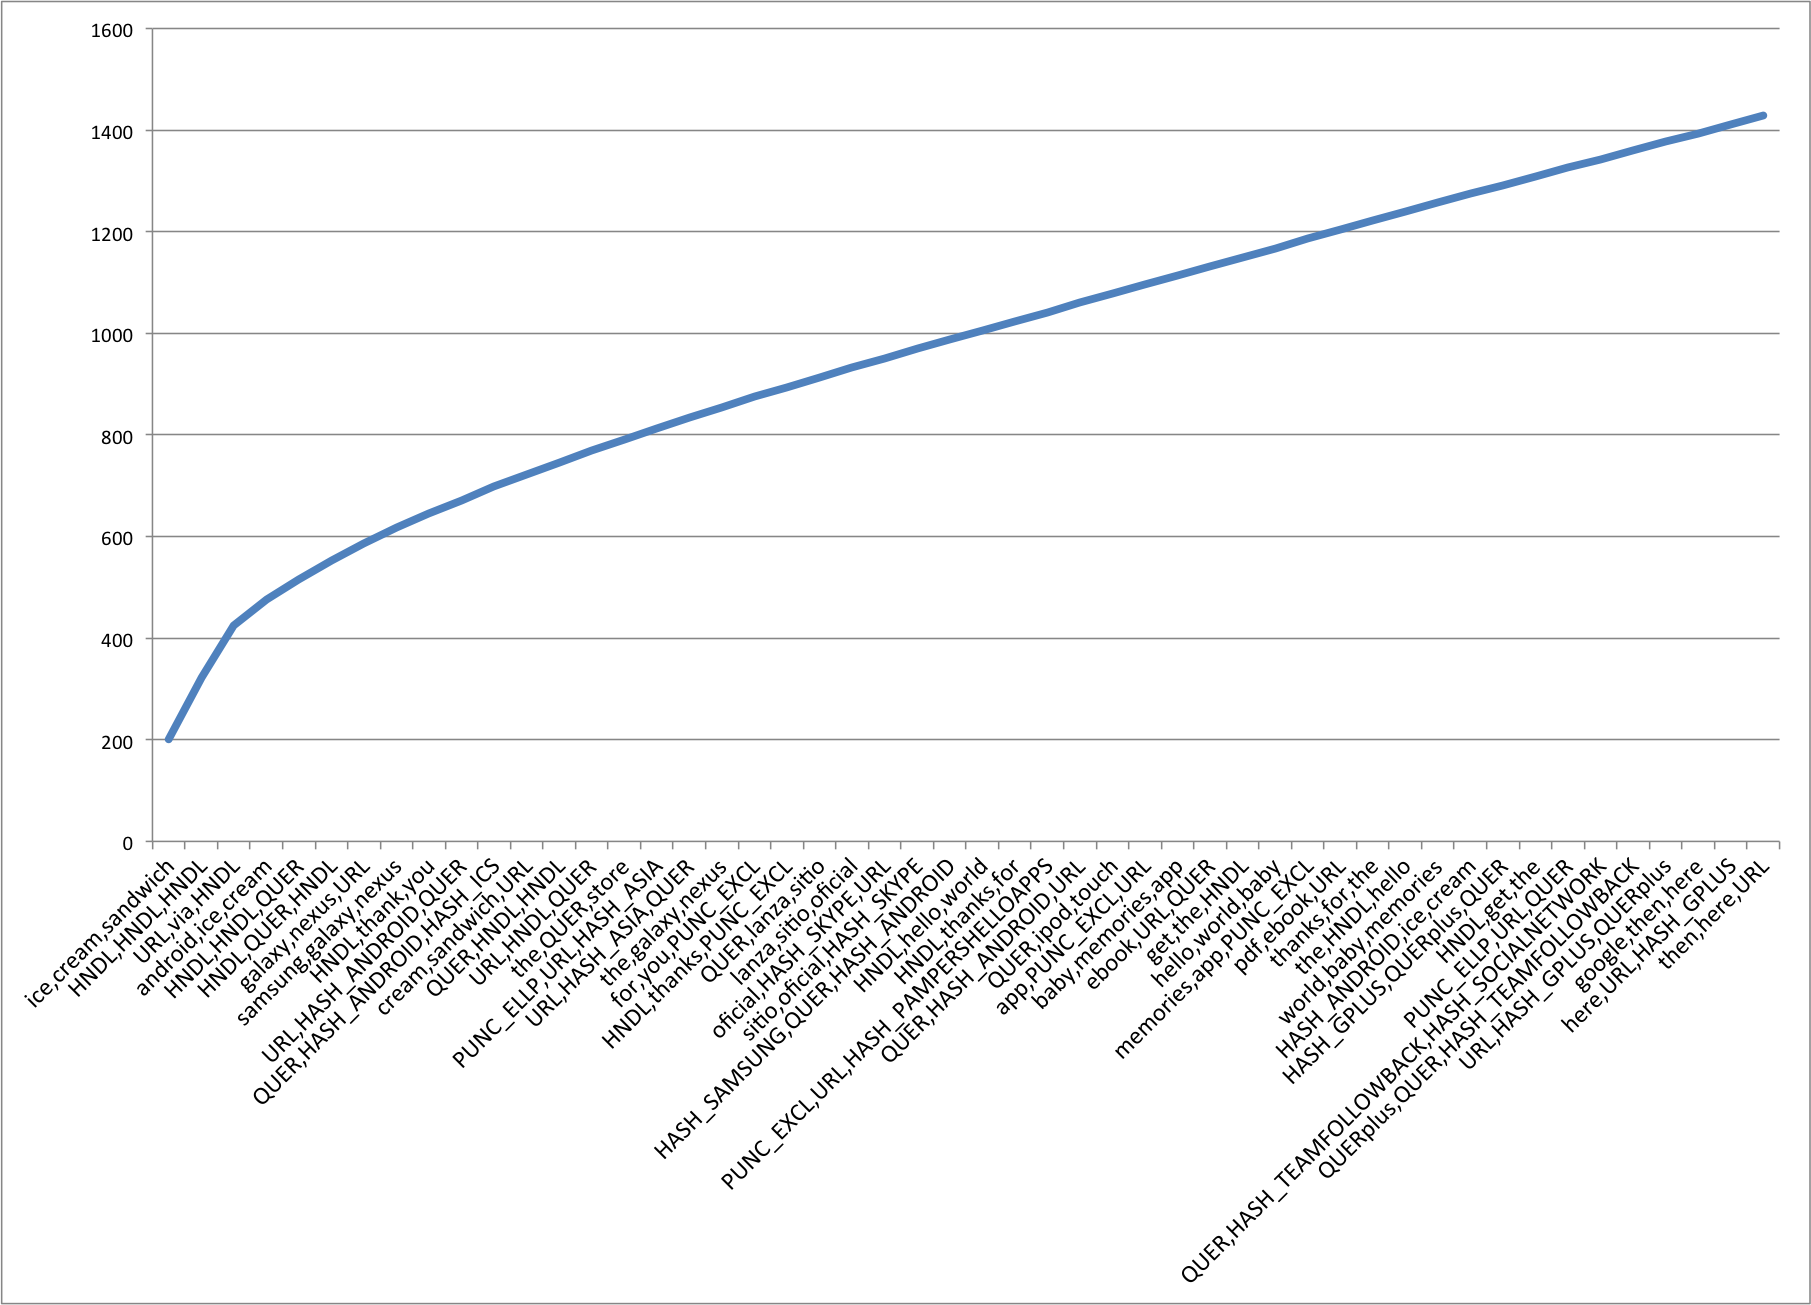
\includegraphics[width=\textwidth]{img/3grams.png}
\caption{Cumulative Frequency Plot for 50 Most Frequent Trigrams}
\label{fig:3grams}
\end{figure}

\subsubsection{Negation Handling} The need negation detection in sentiment
analysis can be illustrated by the difference in the meaning of the phrases,
``This is good'' vs. ``This is not good'' However, the negations occurring in
natural language are seldom so simple. Handling the negation consists of two
tasks – Detection of explicit negation cues and the scope of negation of these
words.

Councill et al. look at whether negation detection is useful for sentiment
analysis and also to what extent is it possible to determine the exact scope of
a negation in the text \cite{CMV}. They describe a method for negation detection
based on Left and Right Distances of a token to the nearest explicit negation
cue.

\subsubsection*{Detection of Explicit Negation Cues} To detect explicit negation
cues, we are looking for the following words in \tabref{tab:negation}. The
search is done using regular expressions.

\begin{table}[h!]
\centering
\begin{tabular}{|l|l|l|}
\hline
S.No. & Negation Cues \\\hline
1.  & never \\
2.  & no \\
3.  & nothing \\
4.  & nowhere \\
5.  & noone \\
6.  & none \\
7.  & not \\
8.  & havent \\
9.  & hasnt \\
10.  & hadnt \\
11.  & cant \\
12.  & couldnt \\
13.  & shouldnt \\
14.  & wont \\
15.  & wouldnt \\
16.  & dont \\
17.  & doesnt \\
18.  & didnt \\
19.  & isnt \\
20.  & arent \\
21.  & aint \\
22.  & Anything ending with ``n't'' \\\hline
\end{tabular}
\caption{Explicit Negation Cues}
\label{tab:negation}
\end{table}

\subsubsection*{Scope of Negation} Words immediately preceding and following the
negation cues are the most negative and the words that come farther away do not
lie in the scope of negation of such cues. We define left and right negativity
of a word as the chances that meaning of that word is actually the opposite.
Left negativity depends on the closest negation cue on the left and similarly
for Right negativity. \figref{fig:negation} illustrates the left and right
negativity of words in a tweet.

\begin{figure}[h!]
\centering
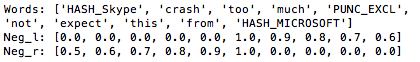
\includegraphics[width=\textwidth]{img/negation.png}
\caption{Scope of Negation}
\label{fig:negation}
\end{figure}
